\setcitestyle{numbers,open={[},close={]}}

Having developed a method and how to implement it, we now apply it to a number of cases of lithium materials.   We choose three common lithium compounds with a variety of properties; metallic lithium, ionic LiF, and covalent $\mathrm{Li_2O}$.  We also analyze a mixed compound obtained after observing beam damage on LiF during a transformation into metallic lithium, which we will also discuss.  

\section{Lithium Oxide}

We begin by investigating $ \mathrm{Li_2O} $.  The calculations were run on a relaxed cell, converged in terms of K points, and RKmax.  Calculations were performed as described in Section \ref{implementation}.   After the initial two calculations, (with no hole then full hole), the density around the excited lithium atom was plotted, see Fig \ref{Li2O_contour}.  The density plots clearly show valence electrons in the material being attracted to the excited atom. This indicates that the core hole should have both a noticeable effect on the final states and that it is screened as well.  We can also see that even the closest lithium atom is largely unaffected by the core hole, in agreement with the supercell size being sufficient to isolate core holes.  Calculating the difference in electron occupancy shows a decrease of 0.88 electron in the basin.  This decrease is smaller then would be expected the no screening limit and according to Eq \ref{final_eq}, indicates that the hole is 12\% screened.  A third calculation was then performed using a decreased hole size to obtain a final spectra.  The ELNES K edge from all three simulations are compared to experiment in Fig \ref{Li2O_three}.  



\begin{figure}
	\centering
	\includegraphics[scale=0.2]{Li2Ocontour_plot}
	\caption{Effect of introducing a core hole in $ \mathrm{Li2O} $.  (a) no hole crystal.  (b) Crystal with hole on starred lithium atom, inducing a response from the valence electrons.  Contour lines on a logarithmic scale. }
	\label{Li2O_contour}
\end{figure}

\begin{figure}
	\centering
	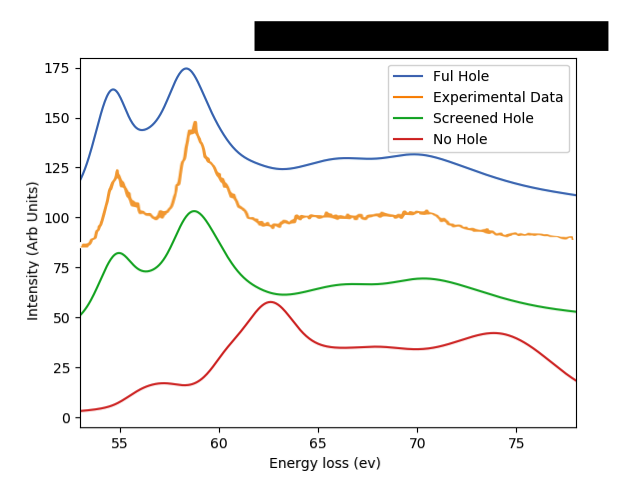
\includegraphics[scale=0.45]{Li2O_three}
	\caption{Lithium K edge of $ \mathrm{Li_2O} $ from the three calculations taken with varying degrees of core hole. }
	\label{Li2O_three}
\end{figure}

\section{Lithium}

\section{LiF}


\newpage
\bibliographystyle{unsrt}


\bibliography{EELS,DFT,EELScalculation,introduction,methods}
